% Niveau :      PC
% Discipline :  Méca
% Mots clés :   Ressort, Impureté, Chaines

\begin{exercise}{Impureté dans un cristal}{2}{Spé}
{Mécanique, Ondes mécaniques, Ressort}{potier,bermu}

On considère une chaîne infinie linéaire d’atomes ponctuels de masse $m$ liés par des ressorts de raideur $K$. La chaîne est portée par l’axe $OX$ ; à l’équilibre, les atomes occupent les positions $x_n = n a$ avec $n\in\mbb{Z}$, où $a$ est la longueur à vide des ressorts. En $X=0$ se trouve une impureté (atome de masse $M$).
\begin{figure}[H]
    \centering
    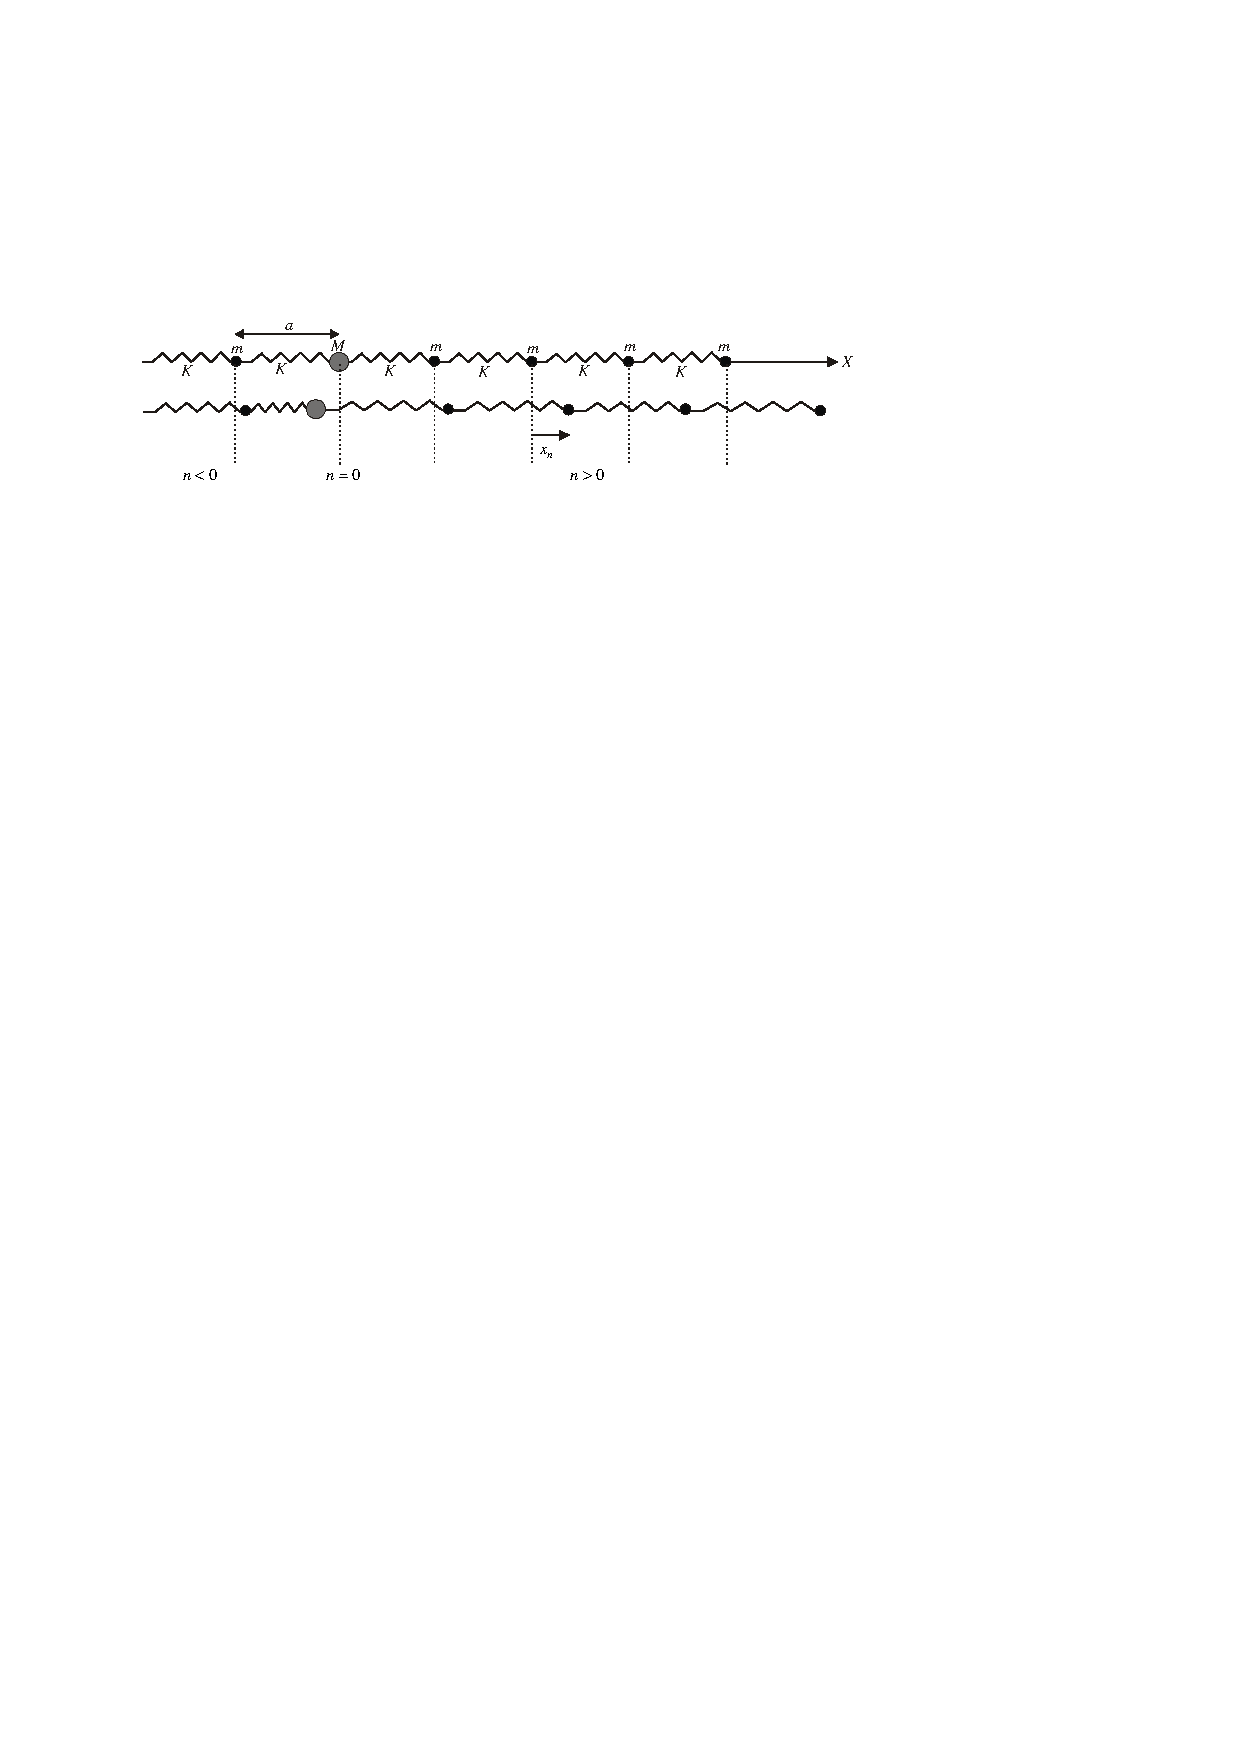
\includegraphics[width=\linewidth]{meca/ondes_meca/impurete.pdf}
    \vspace{-1.5em}
    \caption{Modèle de l'impureté dans un cristal par une chaine de ressorts.}
\end{figure}

\begin{questions}
\question (\emph{Préliminaire}) Quel sens physique peut-on donner à $m$, $K$ et $a$ ? Dans quelle limite le modèle de la chaîne de ressorts est valable ? Estimer en ordre de grandeur ces quantités.
\question Établir le système d'équations différentielles régissant l'écart à l'équilibre $x_n$ de l’atome $n$ par rapport à sa position d’équilibre.

\uplevel{On cherche des solutions sous la forme $\underline{x_n}(t) = A e^{i(\omega t -  k X_n)}$ dans la partie $X_n<0$, avec $A\in\mbb{R}$.}
\question Montrer que $k$ et $\omega$ sont liés par une relation de dispersion.
\question Montrer que si l’on considère une onde progressive incidente $\underline{x_n}(t) = A e^{i(\omega t -  k X_n)}$ dans la partie $X_n<0$, il y a nécessairement en $X=0$ une onde réfléchie d’amplitude $B$ et une onde transmise d’amplitude $C$.\\
Déterminer ces amplitudes complexes en fonction de A.
\question Étudier les cas
\begin{parts}
\part $M \gg m$,
\part $M \ll m$,
\part $\abs{M - m} \ll m, M$.
\end{parts}
Interpréter ces résultats.
\question On se place dans le cas où $M = m$ : il n’y a pas de défaut. \\
Montrer que la chaîne se comporte comme un filtre passe-bas dont on calculera la pulsation de coupure $\omega_c$ . Tracer le graphe $\omega(k)$. \\
On interprétera en particulier $x_n$ dans les cas limites
\begin{parts}
\part $\omega \ll \omega_c$,
\part $\abs{\omega - \omega_c} \ll \omega, \omega_c$.
\end{parts}
\question Déterminer alors la vitesse de phase et la vitesse de groupe
de l’onde. Montrer que l’on peut déterminer dans ce cas une équation d’onde et retrouver les résultats précédents.
\end{questions}
\end{exercise}